\section{Durchschnittsgesicht und Differenzgesichter} \label{sec:facespace}
\begin{tcolorbox}
	\centerline{\textbf{Lernziele Kapitel~\ref{sec:facespace}}}
	\begin{enumerate}[leftmargin=*,label=\thesection.\arabic*]
		\item \label{item:meandiff_simple} Die Lernenden können den Durchschnitt einer Familie von Vektoren von Hand berechnen (für konkrete Zahlenbeispiele).\\
		(Aufgaben~\ref{aufg:meandiff_simple} und~\ref{aufg:meandiff_simple_1})
		\item \label{item:meanface} Die Lernenden können die Addition und Subtraktion von Vektoren und deren Multiplikation mit einem Skalar in Python ausführen.\\
		(Aufgaben~\ref{aufg:meanface} und~\ref{aufg:diffface})
		\item \label{item:hmmc} Die Lernenden können die Begriffe Durchschnittsgesicht und Differenzgesicht erklären.\\
		(Aufgaben~\ref{aufg:difffaces_images} und~\ref{aufg:hmmc})
	\end{enumerate}
\end{tcolorbox}
Wir haben im letzten Kapitel gesehen, dass man Bilder der Auflösung $M\times N$ als Vektoren der Länge $M\cdot N$ auffassen kann.
Diese Vektoren können wir wiederum als Punkte in einem Raum der Dimension $M\cdot N$ auffassen.
In diesem Kapitel werden wir diese Sichtweise ausarbeiten.

Sei $K$ die Anzahl aller Bilder unserer Datenbank.
Jedes Bild soll dabei die Auflösung $M\times N$ haben.
Weiter seien $\vec b_1,\ldots,\vec b_K$ die Vektoren dieser Bilder.
Diese Darstellung erlaubt uns, das \textit{Durchschnittsgesicht}, wir nennen es $\vec m$, zu definieren
\begin{equation*}
	\vec m=\frac{1}{K}\left(\vec b_1+\ldots+\vec b_K\right).
\end{equation*}
Dies ist einfach die Summe der Vektoren dividiert durch deren Anzahl.
Wegen dieser Analogie zum arithmetischen Mittel, nennen wir dies das Durchschnittsgesicht.
Damit können wir die sogenannten \textit{Differenzgesichter} $\vec a_1,\ldots,\vec a_K$ bilden.
Diese sind definiert als als die Verschiebung der Gesichter aus der Datenbank um $-\vec{m}$, also
\begin{equation*}
	\vec a_k=\vec b_k-\vec m,\quad k=1,\ldots,K.
\end{equation*}
Um den Durchschnitt und die Verschiebung von Vektoren geometrisch besser zu verstehen, schauen wir das zuerst in der Ebene an.
\begin{aufgabe} \label{aufg:meandiff_simple}
	Betrachten Sie die folgenden drei Vektoren
	\begin{equation*}
		\vec{b}_1=
		\begin{pmatrix}
			-4 \\
			-5
		\end{pmatrix},\quad
		\vec{b}_2=
		\begin{pmatrix}
			9 \\
			-5
		\end{pmatrix},\quad
		\vec{b}_3=
		\begin{pmatrix}
			1 \\
			7
		\end{pmatrix}.
	\end{equation*}
	\begin{enumerate}[label=(\alph*)]
		\item Berechnen Sie den Durchschnitt $\vec{m}$ der Vektoren $\vec{b}_1,\vec{b}_2,\vec{b}_3$.
		\item \label{item:difference_faces} Berechnen Sie die um $-\vec{m}$ verschobenen Vektoren
		\begin{equation*}
			\vec{a}_1=\vec{b}_1-\vec{m},\quad
			\vec{a}_2=\vec{b}_2-\vec{m},\quad
			\vec{a}_3=\vec{b}_3-\vec{m}.
		\end{equation*}
		\item Zeichnen Sie alle Vektoren $\vec{a}_1,\vec{a}_2,\vec{a}_3$ und $\vec{b}_1,\vec{b}_2,\vec{b}_3$, sowie $\vec{m}$ in ein Koordinatensystem.
	\end{enumerate}
\end{aufgabe}
\begin{losung}
	\begin{enumerate}[label=(\alph*)]
		\item Wie im skalaren Fall ist der Durchschnitt definiert als die Summe geteilt durch dir Anzahl der Summanden, also
		\begin{equation*}
			\vec{m}=\frac{1}{3}\left(\vec{b}_1+\vec{b}_2+\vec{b}_3\right)
			=\frac{1}{3}\left(
			\begin{pmatrix}
				-4 \\
				-5
			\end{pmatrix}+
			\begin{pmatrix}
				9 \\
				-5
			\end{pmatrix}+
			\begin{pmatrix}
				1 \\
				7
			\end{pmatrix}
			\right)
			=
			\begin{pmatrix}
				2 \\
				-1
			\end{pmatrix}.
		\end{equation*}
		\item Für die um $-\vec{m}$ verschobenen Vektoren erhalten wir folglich
		\begin{equation*}
			\vec{a}_1=
			\begin{pmatrix}
				-6 \\
				-4
			\end{pmatrix},\quad
			\vec{a}_2=
			\begin{pmatrix}
				7 \\
				-4
			\end{pmatrix},\quad
			\vec{a}_3=
			\begin{pmatrix}
				-1 \\
				8
			\end{pmatrix}.
		\end{equation*}
		\item Die Skizze ist in Abbildung~\ref{fig:meanddiff_simple} dargestellt.
			Gezeichnet sind die Vektoren aufgefasst als Punkte, also
			\begin{equation*}
				\vec{m}=\overrightarrow{OM},\qquad
				\vec{a}_k=\overrightarrow{OA_k},\qquad
				\vec{b}_k=\overrightarrow{OB_k},\qquad
				k=1,2,3.
			\end{equation*}
			\begin{center}
				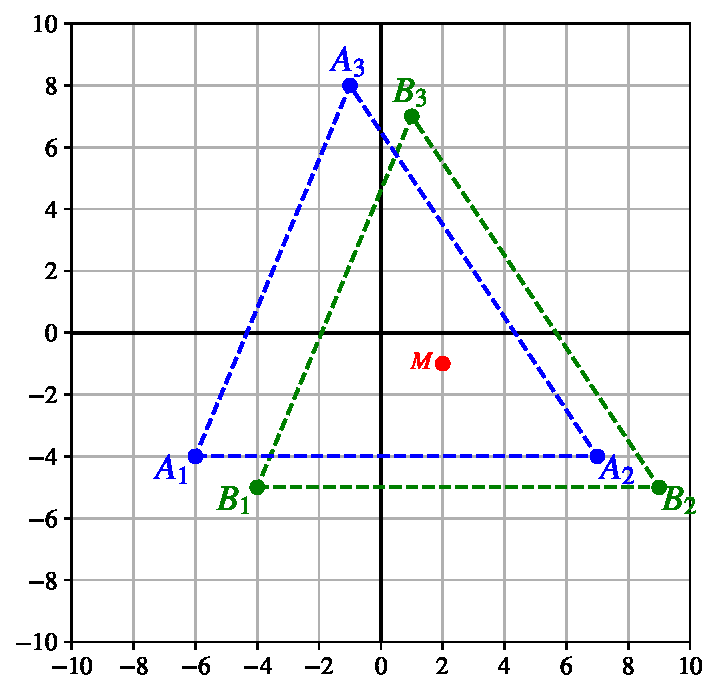
\includegraphics[width=0.5\textwidth]{images/facespace/meandiff_simple}
				\captionof{figure}{Durchschnitt $\vec{m}$ der Vektoren $\vec{b}_1,\vec{b}_2,\vec{b}_3$ sowie deren Translationen $\vec{a}_1,\vec{a}_2,\vec{a}_3$ um $-\vec{m}$, alle aufgefasst als Punkte in der Ebene.}
				\label{fig:meanddiff_simple}
			\end{center}
	\end{enumerate}
\end{losung}
\begin{aufgabe} \label{aufg:meandiff_simple_1}
	Betrachten Sie die Vektoren
	\begin{equation*}
		\vec{b}_1=
		\begin{pmatrix}
			-2 \\
			-1 \\
			1
		\end{pmatrix},\qquad
		\vec{b}_2=
		\begin{pmatrix}
			4 \\
			-1 \\
			1
		\end{pmatrix}.
	\end{equation*}
	\begin{enumerate}[label=(\alph*)]
		\item Berechnen Sie den Durchschnitt $\vec{m}$ der Vektoren $\vec{b}_1$ und $\vec{b}_2$.
		\item Berechnen Sie die um $-\vec{m}$ verschobenen Vektoren
		\begin{equation*}
			\vec{a}_1=\vec{b}_1-\vec{m}
			\qquad\text{und}\qquad
			\vec{a}_2=\vec{b}_2-\vec{m}.
		\end{equation*}
		\item Was ist der Durchschnitt der Vektoren $\vec a_1$ und $\vec a_2$? Was ist der Durchschnitt der Vektoren $\vec a_1,\vec a_2,\vec a_3$ aus Teilaufgabe~\ref{aufg:meandiff_simple}~\ref{item:difference_faces}?
	\end{enumerate}
\end{aufgabe}
\begin{losung}
	\begin{enumerate}[label=(\alph*)]
		\item Wir berechnen die Summe der beiden Vektoren und dividieren durch deren Anzahl
		\begin{equation*}
			\vec{m}=\frac{1}{2}\left(\vec{b}_1+\vec{b}_2\right)
			=\frac{1}{2}\left(
			\begin{pmatrix}
				-2 \\
				-1 \\
				1
			\end{pmatrix}+
			\begin{pmatrix}
				4 \\
				-1 \\
				1
			\end{pmatrix}
			\right)
			=
			\begin{pmatrix}
				1 \\
				-1 \\
				1
			\end{pmatrix}.
		\end{equation*}
		\item Für die um $-\vec{m}$ verschobenen Vektoren erhalten wir folglich
		\begin{equation*}
			\vec{a}_1=
			\begin{pmatrix}
				-3 \\
				0 \\
				0
			\end{pmatrix},\qquad
			\vec{a}_2=
			\begin{pmatrix}
				3 \\
				0 \\
				0
			\end{pmatrix}.
		\end{equation*}
		\item Der Durchschnitt der verschobenen Vektoren ist
		\begin{equation*}
			\frac{1}{2}\left(\vec{a}_1+\vec{a}_2\right)=
			\frac{1}{2}\left(\begin{pmatrix}
				-3 \\
				0 \\
				0
			\end{pmatrix}+
			\begin{pmatrix}
				3 \\
				0 \\
				0
			\end{pmatrix}\right)=
			\begin{pmatrix}
				0 \\
				0 \\
				0
			\end{pmatrix}.
		\end{equation*}
		Wenn man eine Familie von Vektoren um ihren Durchschnitt verschiebt, erhält haben die resultierenden Vektoren immer den Nullvektor als Durchschnitt.
		Folglicht gilt das auch für die Vektoren aus Teilaufgabe~\ref{aufg:meandiff_simple}~\ref{item:difference_faces}.
	\end{enumerate}
\end{losung}
Nun wollen wir das Durchschnittsgesicht
\begin{equation*}
	\vec m=\frac{1}{K}\left(\vec b_1+\ldots+\vec b_K\right)
\end{equation*}
der Bilder aus der Datenbank berechnen und wieder als Bild ausgeben.
Wie sieht so ein Durchschnittsgesicht aus?
Das werden wir in folgender Übung herausfinden.
\begin{aufgabe} \label{aufg:meanface}
	Ergänzen Sie im File \texttt{eigenfaces.py} die Funktion \texttt{meanface(b\_list)}.
	Dabei ist \texttt{b\_list} die Liste der Länge $K$ der Vektoren $\vec b_1,\ldots,\vec b_K$.
	Der Rückgabewert soll das Durchschnittsgesicht $\vec m$ sein.
	Sie können die ihre Lösung überprüfen indem Sie das Skript \texttt{meanface\_test.py} laufen lassen.
	\textit{Hinweis:} Die Python Funktionen \texttt{len(...) und sum(...)} können nützlich sein.
\end{aufgabe}
\begin{losung}
	Hier ist eine mögliche Lösung und das davon mit \texttt{meanface\_test.py} generierte Durchschnittsgesicht.\\[0.5cm]
	\begin{minipage}{0.45\textwidth}
\begin{lstlisting}[style=python]
def meanface(b_list):
	K = len(b_list)
	return sum(b_list) / K
\end{lstlisting}
	\end{minipage}\hfill
	\begin{minipage}{0.3\textwidth}\vspace{-1cm}
		\centering\hfill Durchschnittsgesicht:
	\end{minipage}
	\begin{minipage}{0.2\textwidth}\vspace{-1cm}
		\centering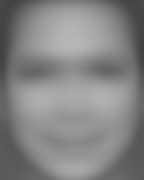
\includegraphics[width=0.6\textwidth]{images/facespace/meanface}
	\end{minipage}
\end{losung}
Nun berechnen wir die \textit{Differenzgesichter} $\vec a_1,\ldots,\vec a_K$, also die Gesichter der Datenbank, welche um $-\vec{m}$ verschoben wurden
\begin{equation*}
	\vec a_k=\vec b_k-\vec m,\quad k=1,\ldots,K.
\end{equation*}
Diese berechnen wir nun in Python.
\begin{aufgabe} \label{aufg:diffface}
	Ergänzen Sie im File \texttt{eigenfaces.py} die Funktion \texttt{diffface(b\_list)}.
	Dabei ist \texttt{b\_list} die Liste der Länge $K$ der Vektoren $\vec b_1,\ldots,\vec b_K$.
	Der Rückgabewert soll eine Liste der Länge $K$ sein, welche die Differenzgesichter $\vec a_1,\ldots,\vec a_K$ gemäss obiger Formel enthält.
	Sie können die ihre Lösung überprüfen indem Sie das Skript \texttt{diffface\_test.py} laufen lassen.
	\textit{Hinweis:} Verwenden Sie die Funktion \texttt{meanface(...)} aus der vorherigen Aufgabe.
\end{aufgabe}
\begin{losung}
	Eine korrekte Lösung könnte so aussehen.
\begin{lstlisting}[style=python]
def diffface(b_list):
	a_list = copy.deepcopy(b_list)
	m = meanface(b_list)
	for k in len(b_list):
		a_list[k] = b_list[k] - m
	return a_list
\end{lstlisting}
\end{losung}
Die eben eingeführten Begriffe sind in Abbildung~\ref{fig:meandiff} für Vektoren mit zwei Komponenten visualisiert.
Die Quintessenz ist, dass sich diese Vektoren (und damit die Bilder) als Punkte in einem Raum der Dimension $M\cdot N$ auffassen lassen.
Wir bezeichnen diese Punkte mit Grossbuchstaben, also ($O$ bezeichnet hier den Ursprung)
\begin{equation*}
	\vec{m}=\overrightarrow{OM},\qquad
	\vec{a}_k=\overrightarrow{OA_k},\qquad
	\vec{b}_k=\overrightarrow{OB_k},\qquad
	k=1,\ldots,K.
\end{equation*}
Die Bilder der Datenbank bilden dann eine \glqq{}Punktewolke\grqq{} in diesem Raum.
Durch Subtraktion von $\vec m$ wir diese Punktewolke um den Ursprung zentriert.
Das Resultat dieser Subtraktion (oder Verschiebung) sind die Differenzgesichter.
Das ist in Abbildung~\ref{fig:meandiff} gezeigt.
\begin{figure}[ht]
	\centering
	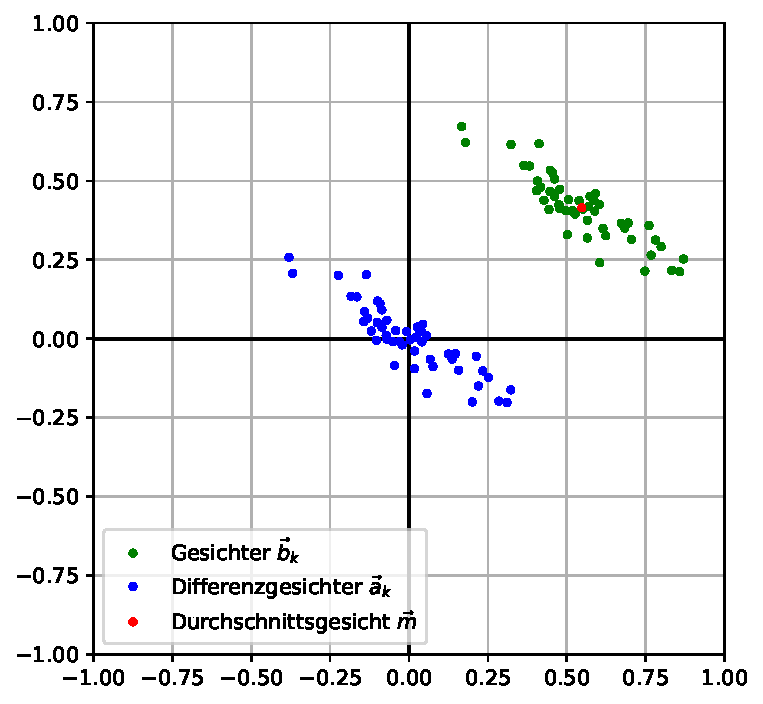
\includegraphics[width=0.5\textwidth]{images/facespace/meandiff}
	\caption{Die Gesichter werden um den Ursprung zentriert indem man das Durchschnittsgesicht subtrahiert.}
	\label{fig:meandiff}
\end{figure}
\begin{aufgabe} \label{aufg:difffaces_images}
	Wir haben in Aufgabe~\ref{aufg:meanface} das Durchschnittsgesicht wieder als Bild dargestellt.
	Könnte man das auch mit den Differenzgesichtern machen?
	Begründen Sie.
\end{aufgabe}
\begin{losung}
	Nein, die Differenzgesichter lassen sich nicht wieder als Bilder darstellen, weil die Einträge dieser Vektoren nicht zwischen 0 und 1 liegen.
	Dies sieht man zum Beispiel in Abbildung~\ref{fig:meandiff}.
	Man kann also diesen Vektor-Einträgen keine Graustufe zuordnen.
\end{losung}
\begin{aufgabe} \label{aufg:hmmc}
	Nennen Sie einen Unterschied und eine Gemeinsamkeit der vereinfachten Darstellung in Abbildung~\ref{fig:meandiff} zu unserer tatsächlichen Situation mit Bildern von Gesichtern.
	Gehen Sie davon aus, dass unsere Bilder eine Auflösung von $M=180$ und $N=144$ haben, wie im letzten Kapitel.
\end{aufgabe}
\begin{losung}
	Als Vektoren aufgefasst sind die Gesichter Punkte im $\mathbb R^{M\cdot N}$.
	Für $M=180$ und $N=144$ wären das Punkte im $\mathbb R^{25'920}$ und nicht im $\mathbb R^2$ wie in der Abbildung.
	Anders ausgedrückt zeigt die Abbildung den Spezialfall $M\cdot N=2$.
	Das entspricht Bilder die nur aus zwei Pixeln bestehen.
	Andererseits wird in der Abbildung korrekt gezeigt, dass die Komponenten der Gesichts-Vektoren $\vec b_k$ nur Werte zwischen 0 und 1 annehmen.
	Zudem sind die Differenzgesichter richtigerweise genau als Verschiebung der Gesichts-Vektoren um $-\vec m$ dargestellt.
\end{losung}
Die Eigengesichter werden nun aus den Differenzgesichtern konstruiert.
Dies wird im nächsten Kapitel behandelt.
%In diesem Kapitel wollen wir diese Punktewolke so verschieben, dass sie um den Ursprung zentriert ist.
%Dazu müssen wir den Durchschnitt (arithmetisches Mittel) dieser Punkte berechnen.
%
%Seien nun $M,N\in\mathbb N$ fix.
%Wir haben im letzten Kapitel gesehen, wie man schwarz-weiss Bilder der Auflösung $M\times N$ als Vektoren in $\mathbb R^{M\cdot N}$ verstehen kann.
%Nun werden wir diese Vektoren als Punkte in einem $M\cdot N$-dimensionalen auffassen.
%Die Bilder der Datenbank bilden dann eine \glqq{}Punktewolke\grqq{} in diesem Raum.
%Wir werden diese Punktewolke nun um den Ursprung zentrieren.
%Dazu benötigen wir das Konzept eines Durchschnitts von Vektoren, welches wir in den 
%
%Die Bilder müssen dafür nicht unbedingt ein Gesicht zeigen.
%Die Pixel können sogar völlig zufällige Graustufen aufweisen, so dass auf dem Bild nichts sinnvolles zu erkennen ist.
%Dies führt uns zu folgender Beobachtung:
%Nur die wenigsten Vektoren in $\mathbb R^{M\cdot N}$ entsprechen einem Gesicht.
%Wir wollen uns näher mit dieser Beobachtung befassen.
%
%Sei $K\in\mathbb N$ die Anzahl aller Bilder von allen Personen unserer Datenbank.
%Jedes Bild soll dabei die Auflösung $M\times N$ haben.
%Wir betrachten alle Bilder der Datenbank als Vektoren $\vec b_1,\ldots,\vec b_K\in\mathbb R^{M\cdot N}$.
%Diese Darstellung erlaubt uns, das \textit{Durchschnittsgesicht}, wir nennen es $\vec m\in\mathbb R^{M\cdot N}$, zu definieren
%\begin{equation*}
%	\vec m=\frac{1}{K}\left(\vec b_1+\ldots+\vec b_K\right).
%\end{equation*}